\documentclass{beamer}

\mode<presentation>
{
  \usetheme{default}
  \usecolortheme{default}
  \usefonttheme{default}
  \setbeamertemplate{navigation symbols}{}
  \setbeamertemplate{caption}[numbered]
  \setbeamertemplate{footline}[page number]
  \setbeamercolor{frametitle}{fg=white}
  \setbeamercolor{footline}{fg=black}
} 

\usepackage[english]{babel}
\usepackage[utf8x]{inputenc}
\usepackage{tikz}
\usepackage{listings}
\usepackage{courier}
\usepackage{array}
\usepackage{bold-extra}
\usepackage{minted}

\xdefinecolor{darkblue}{rgb}{0.1,0.1,0.7}
\xdefinecolor{darkgreen}{rgb}{0,0.5,0}
\xdefinecolor{darkgrey}{rgb}{0.35,0.35,0.35}
\xdefinecolor{darkorange}{rgb}{0.8,0.5,0}
\xdefinecolor{darkred}{rgb}{0.7,0,0}
\xdefinecolor{dianablue}{rgb}{0.18,0.24,0.31}
\definecolor{commentgreen}{rgb}{0,0.6,0}
\definecolor{stringmauve}{rgb}{0.58,0,0.82}

\lstset{ %
  backgroundcolor=\color{white},      % choose the background color
  basicstyle=\ttfamily\small,         % size of fonts used for the code
  breaklines=true,                    % automatic line breaking only at whitespace
  captionpos=b,                       % sets the caption-position to bottom
  commentstyle=\color{commentgreen},  % comment style
  escapeinside={\%*}{*)},             % if you want to add LaTeX within your code
  keywordstyle=\color{blue},          % keyword style
  stringstyle=\color{stringmauve},    % string literal style
  showstringspaces=false,
  showlines=true
}

\lstdefinelanguage{scala}{
  morekeywords={abstract,case,catch,class,def,%
    do,else,extends,false,final,finally,%
    for,if,implicit,import,match,mixin,%
    new,null,object,override,package,%
    private,protected,requires,return,sealed,%
    super,this,throw,trait,true,try,%
    type,val,var,while,with,yield},
  otherkeywords={=>,<-,<\%,<:,>:,\#,@},
  sensitive=true,
  morecomment=[l]{//},
  morecomment=[n]{/*}{*/},
  morestring=[b]",
  morestring=[b]',
  morestring=[b]"""
}

\title[2017-06-23-root-numpyinterface]{BulkIO $\to$ Numpy, progress and performance}
\author{Jim Pivarski}
\institute{Princeton University -- DIANA}
\date{June 23, 2017}

\begin{document}

\logo{\pgfputat{\pgfxy(0.11, 8)}{\pgfbox[right,base]{\tikz{\filldraw[fill=dianablue, draw=none] (0 cm, 0 cm) rectangle (50 cm, 1 cm);}}}\pgfputat{\pgfxy(0.11, -0.6)}{\pgfbox[right,base]{\tikz{\filldraw[fill=dianablue, draw=none] (0 cm, 0 cm) rectangle (50 cm, 1 cm);}
\includegraphics[height=0.99 cm]{diana-hep-logo.png}\tikz{\filldraw[fill=dianablue, draw=none] (0 cm, 0 cm) rectangle (4.9 cm, 1 cm);}}}}

\begin{frame}
  \titlepage
\end{frame}

\logo{\pgfputat{\pgfxy(0.11, 8)}{\pgfbox[right,base]{\tikz{\filldraw[fill=dianablue, draw=none] (0 cm, 0 cm) rectangle (50 cm, 1 cm);}
\includegraphics[height=1 cm]{diana-hep-logo.png}}}}

% Uncomment these lines for an automatically generated outline.
%\begin{frame}{Outline}
%  \tableofcontents
%\end{frame}

%%%%%%%%%%%%%%%%%%%%%%%%%%%%%%%%%%%%%%%%%%%%%%%%%%%%%%%

\begin{frame}{Purpose of this project}
\vspace{0.5 cm}

\textcolor{darkblue}{\large To give native Numpy support to ROOT.}

\vspace{0.5 cm}
Potential aspects:
\begin{enumerate}
\item TTree branches $\to$ Numpy arrays.
\item Numpy arrays $\to$ TTree branches.
\item PyROOT {\tt\small ROOT.std.vector} (etc.) $\to$ Numpy.
\end{enumerate}

\vspace{0.5 cm}
This talk addresses only \textcolor{darkblue}{\#1}, but the others aren't off the table.
\end{frame}

\begin{frame}{Why? Isn't there a root\_numpy?}
\vspace{0.5 cm}
\large

root\_numpy is an external project that uses Cython and TTreeFormula to fill Numpy arrays.

\vspace{0.5 cm}
We want Numpy support
\begin{itemize}
\item to be a part of ROOT (to streamline interaction with machine learning libraries, for instance),
\item without unnecessary dependencies (Numpy only),
\item taking advantage of ROOT internals for performance.
\end{itemize}

\vspace{0.5 cm}
\uncover<2->{\textcolor{darkblue}{In fact, this is a great application of Brian's BulkIO.}}
\end{frame}

\begin{frame}{Scope of TTree branches $\to$ Numpy arrays}
\vspace{0.5 cm}
\large
\begin{itemize}\setlength{\itemsep}{0.25 cm}
\item<1-> A single-leaf branch becomes a Numpy array.

\vspace{0.15 cm}
\begin{itemize}\setlength{\itemsep}{0.25 cm}
\item<2-> Multidimensional leaves (with ``{\tt[\ldots]}'' in the title) affect the {\it shape} (dimensionality) of the array--- one-to-one with TLeaf.
\item<3-> Variable length leaves (with ``{\tt[counter]}'' in the title) require the counter to be read and maybe returned to the user.
\end{itemize}

\item<4-> A ``leaf-list'' branch becomes a Numpy {\it record array} (like an array of C structs: row-wise, can't have different lengths, can manually set the byte offsets).

\item<5-> A branch with subbranches becomes a Python dictionary of Numpy arrays.

\item<6-> No attempt to reconstruct objects from the branch data; \\ I have a separate project to do this in Python.
\end{itemize}
\end{frame}

\begin{frame}[fragile]{Implemented interface (low level)}
\vspace{0.5 cm}

\small
\begin{minted}{python}
ROOT._numpyinterface.iterate(*branches,
                             return_new_buffers=True,
                             swap_bytes=True)
\end{minted}
\normalsize

\begin{itemize}
\item<1-> Returns an iterator over clusters, yielding
\small
\begin{minted}{python}
(entry_start, entry_end, array, array, array...)
\end{minted}
\normalsize for each cluster.

\item<2-> {\tt\small return\_new\_buffers} determines whether arrays are read-only views of ROOT's internal data or are copies. Default is to copy to discourage accidental abuse.

\item<3-> If all baskets align per cluster, zero-copy is possible. Otherwise, we need to double-buffer to match entry ranges.

\item<4-> {\tt\small swap\_bytes} transforms to little endian; in either case, the correct Numpy flag is set.
\end{itemize}
\end{frame}

\begin{frame}[fragile]{Implemented interface (low level)}
\vspace{0.5 cm}
\small
\begin{minted}{python}
ROOT._numpyinterface.dtypeshape(*branches,
                                swap_bytes=True)
\end{minted}
\normalsize

\begin{itemize}
\item Just get the types and lengths and do not iterate.

\item Useful for setting up allocate-then-fill with the iterator.
\end{itemize}
\end{frame}

\begin{frame}[fragile]{Implemented interface (high level)}
\vspace{0.5 cm}
\small
\begin{minted}{python}
ROOT.numpyinterface.arraydict(*branches,
    allocate = lambda shape, dtype:
                   numpy.empty(shape, dtype=dtype),
    trim = lambda array, length: array[:length],
    swap_bytes = True)
\end{minted}
\normalsize
\begin{itemize}
\item High-level interface to filling arrays with overridable allocators.
\item Have to trim {\tt\small dtypeshape}'s overestimate.
\end{itemize}

\vspace{0.25 cm}
\begin{uncoverenv}<2->
\small
\begin{minted}{python}
ROOT.numpyinterface.recarray(*branches,
                             swap_bytes = True)
ROOT.numpyinterface.iterate_pandas(*branches)
ROOT.numpyinterface.pandas(*branches)
\end{minted}
\normalsize
\begin{itemize}
\item Maybe PyTables (for HDF5), etc.
\item All implemented in Python for import-flexibility.
\end{itemize}
\end{uncoverenv}
\end{frame}

\begin{frame}{First page}
\vspace{0.5 cm}
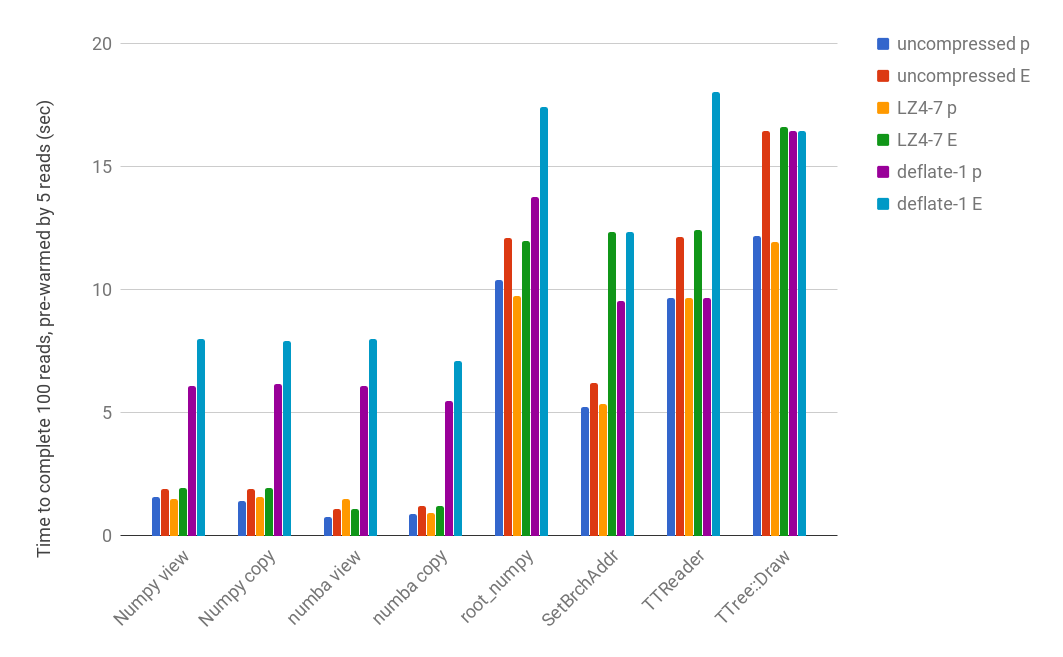
\includegraphics[width=1.1\linewidth]{chart.png}
\end{frame}

\end{document}
